\documentclass{article}
\usepackage[utf8]{inputenc}
\usepackage{listings}
\usepackage{amsmath}
\usepackage{wasysym}
\usepackage{amssymb}
\usepackage{xcolor}
\usepackage{tabularx}
\usepackage[ruled,vlined,linesnumbered]{algorithm2e}
\usepackage{tikz}
\usepackage{hyperref}

\newcommand{\todo}[1]{\textcolor{red}{$\star$~TODO: \textbf{#1}}}
\newcommand{\R}{\mathbb{R}}
\newcommand{\randint}{\operatorname{RANDINT}}
% \newcommand{\argmin}[1]{\operatorname{argmin}\limits_{#1}}
\DeclareMathOperator*{\argmin}{argmin}

\newcommand{\bb}[1]{\textbf{#1}}
\newcommand{\uu}[1]{\underline{#1}}
\newcommand{\ii}[1]{\textit{#1}}

\newenvironment{pyc}{\begin{lstlisting}[language=Python]}{\end{lstlisting}}
\newcommand{\py}[1]{\lstinline[language=Python]{#1}}

\newcommand{\vertex}[1]{\filldraw [black] (#1) circle (1.5mm);}

\renewcommand{\thesection}{\Alph{section}}
\setcounter{section}{2}
% \renewcommand{\thealgocf}{}


\title{IADS Coursework 3}
\author{Samo Nov\'ak (s1865783)}
\date{March 2020}

\begin{document}

\maketitle

\section{Algorithm: Nearest Neighbour Insertion}

\todo{Name? Call it \bb{expansion}?}

We draw inspiration for this algorithm from the outline of Nearest Insertion
(and other TSP heuristics) by Nilsson\cite{nilsson}. We chose this particular
algorithm because of its elegance -- it follows a very simple principle:
start with some trivial circuit of minimum weight and then find the most suitable
nodes to add to it, until all nodes are used. The pseudocode for this algorithm is
presented below, as is some more discussion and visual explanation. In the program
submitted, this is \py{Graph.NearestExpand()}.
\\

\begin{algorithm}[H]
  \KwIn{an undirected complete graph $G=(V,E)$, where $|V| = n$}
  \KwIn{a weight function $w:V\times V \to \mathbb{R}^{+}$,
    note: $\forall v\in V \ldotp w(v,v) = 0$}
  \KwResult{a permutation $\pi$ (represented as list) of
    all vertices representing a circuit (the path the travelling salesperson will take)}

  Initialize: $\pi \gets [i,j]$, where $(i,j)=\argmin_{(i,j)\in E} w(i,j)$ \nllabel{init-pi}
  \tcc*{$\Theta(n^2)$}
  
  Initialize: $U = \{ x\in V | x \notin \pi \}$ \nllabel{init-unused}
  \tcc*{$\Theta(n)$}
  \While{$U \ne \varnothing$  \tcc*{cycle will run $n-2 = \Theta(n)$ times}}{
    $(i, u)\gets \argmin_{(i,v):\;i\in\{0,...,|\pi|-1\},\;v\in U}
    \left\{w\left(\pi[i], v\right)\right\}$ \nllabel{argmin-iu}
    \tcc*{$\Theta\left( n \right)$}
    
    $d_{-} \gets w\left( u, \pi\left[(i-1) \mod |\pi|\right] \right)$
    \nllabel{dminus} \tcc*{$\Theta(1)$}
    
    $d_{+} \gets w\left( u, \pi\left[(i+1) \mod |\pi|\right] \right)$
    \nllabel{dplus} \tcc*{$\Theta(1)$}
    
    \eIf{$d_{-} < d_{+}$ \nllabel{choose-insertion-point} \tcc*{$\Theta(1)$}}{
      Insert $u$ into $\pi$ at position $i$
      \tcc*{$\Theta(n)$}
    }{
      Insert $u$ into $\pi$ after position $i$, so at
      position $(i+1)\mod|\pi|$
      \tcc*{$\Theta(n)$}
    }
    Remove $u$ from $U$. \tcc*{$O(n)$ (impl. dep.)}
  }
  \KwRet{$\pi$}\;
  \caption{Nearest Insert}
\end{algorithm}

On line~\ref*{init-pi}, we initialize the permutation $\pi$ to a list of two nodes
$i,j$, such that their distance $w(i,j)$ in the graph is minimal. We also intialize
a set $U$ of nodes \ii{yet unused} in $\pi$ (line~\ref*{init-unused}).

We shall repeat the following steps \bb{while} $U$ is not empty, meaning $\pi$
does not contain all the nodes. First we need to find the nearest neighbour
(an unused node) $u$ to some node contained in $\pi$ (at index $i$). We do this
by looking for a pair where first element is the index in $\pi$ and the second is
an unused node, such that the nodes $u$ and $\pi[i]$ have minimal distance
(line~\ref*{argmin-iu}).

Next, we need to decide where to place the new node $u$. We know, that its distance to
$\pi[i]$ is minimal, but there are two ways to insert it into $\pi$: before $\pi[i]$
or after it. Therefore, we need to compare the distances to the predecessor and
successor of $\pi[i]$ in the permutation. We use $\pi[(i\pm 1)\mod|\pi|]$
(lines~\ref*{dminus},~\ref*{dplus}), because the salesperson's walk is a cycle,
so the first and last node in $\pi$ are connected as well. We then choose the lower
distance, because we want to minimize the weight of the permutation overall.
(\bb{if} statement starting at line~\ref*{choose-insertion-point})

After inserting $u$ at the appropriate position, we remove it from $U$ -- we wouldn't want
to insert the same node multiple times. We also like our algorithms to terminate.

The running time of this algorithm is $\Theta(n^2)$, where $n=|V|$. This comes
from the fact that the most significant contributions are done by the $\Theta(n^2)$
terms. The running time of lines \ref*{init-pi}, \ref*{init-unused}, \ref*{argmin-iu}
will be elaborated on in the Appendix~\ref{appendix:runtime-ni}, in the interest of
preserving clarity in this section.

Below is a simple visualisation of the described algorithm. We have used a 2-D
Euclidean graph for the visualisation, because it will be easy to see distances
intuitively.
\\

\begin{figure}[h]
  \begin{tikzpicture}[scale=.5,auto=left]
    \vertex{1,3};
    \vertex{3,1};
    \vertex{3,5};
    \vertex{4,1};
    \vertex{4,3};

    \draw[dashed] (3,1) -- (4,1);
  \end{tikzpicture}
  \hspace{1.5cm}
  \begin{tikzpicture}[scale=.5,auto=left]
    \vertex{1,3};
    \vertex{3,1};
    \vertex{3,5};
    \vertex{4,1};
    \vertex{4,3};

    \draw (3,1) -- (4,1);
  \end{tikzpicture}
  \hspace{1.5cm}
  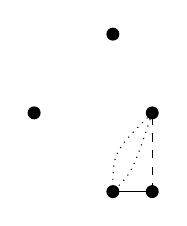
\begin{tikzpicture}[scale=.5,auto=left]
    \vertex{1,3};
    \vertex{3,1};
    \vertex{3,5};
    \vertex{4,1};
    \vertex{4,3};

    \draw (3,1) -- (4,1);
    \draw[dashed] (4,1) -- (4,3);
    \draw[dotted] (4,3) .. controls (3,2) and (3,2) .. (3,1);
    \draw[dotted] (4,3) .. controls (3.5,1.5) and (3.5,1.5) .. (3,1);
  \end{tikzpicture}
  \hspace{1.5cm}
  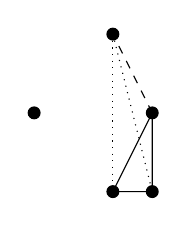
\begin{tikzpicture}[scale=.5,auto=left]
    \vertex{1,3};
    \vertex{3,1};
    \vertex{3,5};
    \vertex{4,1};
    \vertex{4,3};

    \draw (3,1) -- (4,1) -- (4,3) -- (3,1);
    \draw[dashed] (4,3) -- (3,5);
    \draw[dotted] (3,5) -- (3,1);
    \draw[dotted] (3,5) -- (4,1);
  \end{tikzpicture}
  \caption{aaa}
\end{figure}



\section{Experiments}

In this part, we were to generate (or write a generator for) many different
test cases and quantitatively measure how each heuristic (Swap, 2-Opt,
Greedy, \todo{own}) performs.

\subsection{Test generation}

Firstly, let us summarize the assumptions and setting of the problem:
\begin{itemize}
\item We have an \uu{undirected}, \uu{complete} graph $G=(V,E)$ where $|V|=n$.
\item We have a weight function $w:V\times V\to\R^{+}$, such that
  $\forall i,j\in V \ldotp w(i,j) = w(j,i)$, which will be represented as
  a \uu{symmetric} matrix \py{Graph.dists[i][j]}\,$= w(i,j)$).
  We assume $\forall i\in V\ldotp w(i,i)=0$.
\item We have three cases of our problem: \uu{general} TSP
  (no other constraints), \uu{metric} TSP ($w$ is a metric, so
  $\forall u,v,x\in V\ldotp w(u,v)\le w(u,x) + w(x,v)$), and
  \uu{Euclidean} TSP (the graph is embedded in a plane, this is also metric).
\end{itemize}

The test cases could be generated as completely random graphs. For small graphs
(\todo{how big?}), it is then feasible to compute the best path, so that we can
compare it to the results from the tested heuristics. However, for larger graphs,
it will be more useful to generate a graph with some pre-planned best path.

\subsubsection{Small random graphs}

Generating these will be simple: we shall populate the matrix
\py{Graph.dists} with random positive integers. Then we will
compute the best TSP path.

In the \uu{Euclidean} case, we will instead generate randomly positioned
cities in a plane.

For a general \uu{metric} case, we will generate the cities randomly embedded
in a plane, same as in the Euclidean case. However, we will use
the \uu{taxicab} metric (also called the \uu{Manhattan} metric), which measures
the distance along the axes individually and sums them. In the case of discrete
positions (which we will use):
\begin{align*}
  & w_M: \mathbb{N}^d \times \mathbb{N}^d \to \mathbb{N} \\
  & w_M\left(\left<u_1,...,u_d\right>, \left<v_1,...,v_d\right>\right) = \sum_{i=1}^d \left|u_i - v_i\right|
\end{align*}
where $d$ is the number of dimensions of the space (in our case $d=2$
\todo{more dimensions??}).

Since all these graphs will be small, we can get the optimal TSP solution by
simply trying out all the permutations.

\subsubsection{Larger graphs}

A good way to intentionally generate an optimal path in a graph is to create
a cycle with small weights in it and then assign larger values to all the other
edges. So:
\begin{align*}\forall i\in\{0,...,n-2\}\ldotp w(i,i+1) & =\randint(1,5)\\
  \forall i,j\in{0,...,n-1}\ldotp i\ne j \wedge j\ne i+1 \ldotp
  w(i,j) & = \randint(6,10) \\
\end{align*}
The random number boundaries here are somewhat arbitrary, we just need to make
sure that the cycle has smaller values.

Once we have this matrix, we swap the vertices around, so that the initial
permutation $[0,1,...,n-1]$ won't immediately be the solution.


\appendix
\renewcommand{\thesection}{$\Omega$\roman{section}}
\section{Running time of Nearest Insert}
\label{appendix:runtime-ni}


\bibliographystyle{abbrv}
\begin{thebibliography}{9}
\bibitem{nilsson}
  Christian Nilsson,
  \textit{Heuristics for the Traveling Salesman Problem},
  Link\"oping University,
  2003.
  Accessible online [27-03-2020]: \url{https://pdfs.semanticscholar.org/7b80/bfc1c5dd4e10ec807c6f56d0f31f8bf86bc6.pdf}
\end{thebibliography}

\end{document}
